\documentclass[letterpaper]{article}
\usepackage{natbib,alifeconf}
\usepackage{epstopdf}
\usepackage{amsmath}

\title{Model of evolution and self-learning based on predictor neural networks}
\author{Konstantin Lakhman \and Mikhail Burtsev \\
\mbox{}\\
Neuromorphic Cognitive Systems Lab, Kurchatov NBICS-Centre, \\
National Research Center ``Kurchatov Institute'', 1 Kurchatov sqr., Moscow, Russia \\
klakhman@gmail.com}

\begin{document}
\maketitle

\begin{abstract}
	Predictor neural networks is an innovative model for self-learning.
\end{abstract}

\section{Introduction}

\section{Model}

\subsection{Overview}

The proposed model for the generation of the neuromorphic controller consists of the three main blocks: evolutionary algorithm, development algorithm and algorithm for self-learning during the agent's life (Fig.~\ref{Model_Overview}).

We used neuroevolutionary model based on duplications and divergence of neurons' functional roles~\citep{LakhmanBurtsev2013}. We had to adapt this principle because in the current research the topology of neuromorphic controller is not directly encoded in the genome of the agent.  
Instead, genome is a network consists of so-called {\em neuronal pools}, and controller's structure is determined during the development process.

\begin{figure}[b!]
\begin{center}
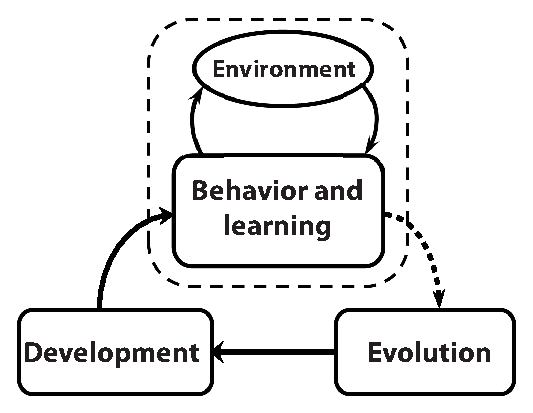
\includegraphics[width=6cm]{Fig1_Model_Overview.eps}
%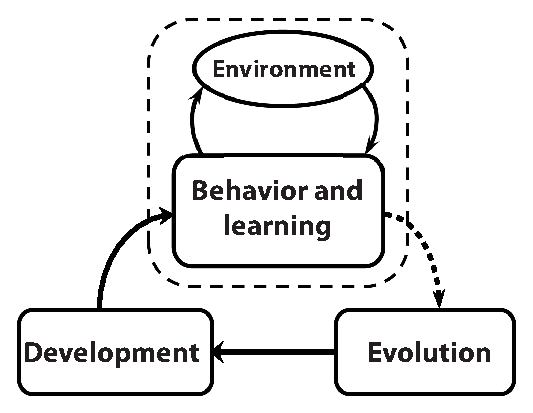
\epsfig{file=Fig1_Model_Overview.eps, width=8.4cm}
\caption{Schematic representation of the model's components}
\label{Model_Overview}
\end{center}
\end{figure}

According to the neuronal group selection theory~\citep{Edelman1993} development algorithm implements two different objectives: generation of a primary repertoire of behavior and generation of a {\em ``diversity of repertoires''} required for further self-learning during life. During the developmental process agent's genotype (network of neuronal pools) translates into phenotype, i.e. the controller providing the agent's behavior in the environment. Groups of neurons are encoded in the genome via the neuronal pools notion. Neurons from the same pool construct similar but not identical connections with the rest of the network. The most connected parts of the network are determined via stochastic endogenous activations of neurons in the isolation from model environment. These parts will be active in the very beginning of the agent's life. The remaining parts of the network form a set of {\em silent neurons} that will be used for further learning.     

Behavior in accordance with the theory of functional systems~\citep{Anokhin1974} occurs in three stages: generation of an action and prediction of the result; evaluation of the action result; formation of the new functional systems of neurons if additional leaning is needed. We present realizations of these phases on the level of individual neurons of the controller. Controller's neural network structure consists of two types of connections between neurons: effector synapses and {\em predictor synapses}. Effector synapses correspond to the standard connections in the theory of artificial neural networks, that transmit excitation between neurons. Predictor synapses do not serve for the excitation propagation and are used by neurons to generate prediction of its future activity. Moments of the {\em mismatch} between agent's actions and environment are detected in the case of discrepancy of formed prediction and observed activity of the neurons. It is necessary to conduct learning procedure at such a moments. This procedure includes activation of the silent neurons, that specialize to modify agent's behavior in the problematic states of the environment via special organization of their connectivity structure. Agent's ability to generate meaningful and useful prediction at the neuronal level is subject to selection process of the predictor connections in the course of evolution.

\subsection{Environment with hierarchy of goals and agent's controller}

We used hypercubic environment~\citep{LakhmanBurtsev2013} as the model environment, where a population of agents evolves. Here we give only a brief description of this model and a concept of goals in it. State of the environment is represented as a binary string and at each discrete time step the agent performs an action -- changing the state of the one bit of this string. Thus agent is moving along edges of the hypercube. The goal in this environment is defined as the consecutive changes of a particular bits of the state vector. Set of such a goals in the environment forms a branched hierarchy: one goal could be nested in another one, i.e. be a beginning of it, and two different goals could have identical nested goal.     

Agent operates in the environment for a fixed amount of time, performs actions and therefore achieves various goals. Fixed reward is associated with each goal, that affects the reproductive success of an agent in the evolution. However, in contrast to paper~\citep{LakhmanBurtsev2013} we have changed the mechanism of reward's recovery in case when the agent attempts to repeatedly reach the same goal in a short amount of time -- recovery period of a goal. Previously, the reward associated with a goal after it's achieving was reseted to zero level and then linearly recovered to its initial value. In the current research we had to introduce the mechanism, which would allow the agent to obtain information about the success in the goals' achievement. With this purpose we {\em ``restrict''} the agent in the achieving not fully restored goal. If the agent was trying to perform an action that would lead to the achievement of the unrestored goal, we blocked the change of the bit and the state vector of the environment remained the same. Thus, the agent should develop a correct interpretation mechanism of such a situations in the course of evolution. 

Agent's behavior in the environment is controlled by a neural network. The structure of this neurocontroller is determined by a processes of evolution, development and learning. The controller consists of three types of neurons: input, output and interneurons. Number of input and output neurons is fixed and determined by a dimension $n^{\mathrm{env}}$ of the hypercubic environment (within this study we used environments with 8 bits dimension). Input neurons are used to transmit the information about current state vector into the network, so input layer has one neuron for each bit. Output neurons encode action that agent performs on a current discrete time step. Each pair of output neurons is responsible for turning on or off a particular bit of the state vector. Current agent's action are selected according to the pair of the most active output neurons. Thus, the number of output neurons is determined as:

\begin{equation}
	n^{out}=\underset{n}{\operatorname{argmin}} \left[\dbinom{2}{n}\geq2n^{env}\right] \enspace . 
\end{equation}   

Interneurons of neurocontroller are organized in a layered topology, which in general case has no restriction on its connectivity structure. This allows to form both direct and recurrent effector synapses. As usual excitation propagates by recurrent effector synapses with unit time delay.

\subsection{Evolutionary algorithm}

Genotype of an agent is a triple (network with two types of connections):

\begin{equation}
	G = \left( P, EC, PC\right)\enspace , 
\end{equation} 

\noindent where $P = \left\{P_{\alpha}\right\}$ is a set of network's neuronal pools, $EC = \left\{ec_{\gamma\alpha}\right\}$ is a set of of effector connections between pools, $PC = \left\{pc_{\gamma\alpha}\right\}$ is a set of predictor connections. During the development process this genotype are used to construct neuromorphic system that will control agent's behavior and provide learning. Each neuronal pool $P_{\alpha}$ in the genotype corresponds to a group of neurons with similar connectivity topology and has the following parameters: {\em a)} pool's size $c_{\alpha}$, i.e. the number of neurons that will be formed from this pool during development; {\em b)} mean $m_{\alpha}$ and standard deviation $\sigma_{\alpha}$ of the biases of the neurons, that corresponds to a particular pool.

Each effector connection $ec_{\gamma\alpha}$ between pools $\alpha$ and $\gamma$ has the following parameters:  {\em a)} mean $m_{\gamma\alpha}$ and standard deviation $\sigma_{\gamma\alpha}$ of the weights of the synapses, that will be formed between neurons belonging to the corresponding pools; {\em b)} probability of the synapse development $p^{\mathrm{dev}}\left(ec_{\gamma\alpha}\right)$.

Predictor connections $pc_{\gamma\alpha}$ have only one attribute -- the probability of connection development $p^{\mathrm{dev}}\left(pc_{\gamma\alpha}\right)$ (by analogy with effector connections).

Population of an agents with controller, resulting from a translation of a described genomes, are placed in the environment to determine their effectiveness. The success of each agent is calculated as the total amount of rewards, which it could collect for a fixed amount of time. Reproductive success of the agent, i.e. the probability to be selected as the parent for the next population, is directly proportional to the agent's effectiveness. Each selected parent goes through a number of mutations, among which are mutations of all numerical parameters of the genome introduced above, to produce an offspring. We used {\em duplication pool} mutation described in detail in the paper~\citep{LakhmanBurtsev2013} as the main structural mutation. This mutation implies formation of a two pools with the same connectivity structure and half the size from a single ``parent'' pool. We also used addition and deletion of both types of connections as additional structural mutations. Full list of numerical parameters of mutations that have been used for the simulation is provided in the Appendix A.

\subsection{Development algorithm}

Developmental algorithm used in this paper consists of three phases: construction of a complete neuromorphic network, simulation of a stochastic version of a network isolated from the model environment, selection of the network's structural elements according to the numerical indicators obtained during the simulation.

\subsubsection{Formation of neurocontroller} During the process of constructing a complete network each neuronal pool is translated into a fixed number of neurons determined by the size $c_{\alpha}$ of the corresponding pool $P_{\alpha}$. Bias $b_{i}$ of each neuron $v_{i}$ is determined according to the normal distribution: $b_{i}\sim \mathcal{N} \left(m_{\alpha},\sigma^2_{\alpha}\right), \enspace \alpha : v_{i} \in P_{\alpha}$. Effector synapses between constructed neurons are determined in accordance with the structure of effector connections in the genome. $\forall \alpha, \beta, i, j : v_{i} \in P_{\alpha}, v_{j} \in P_{\beta} \rightarrow w_{ji} \sim \mathcal{N} \left(m_{\beta\alpha},\sigma^2_{\beta\alpha}\right),\enspace \mbox{if} \enspace ec_{\beta\alpha} \in EC \enspace \mbox{with probability} \enspace p^{\mathrm{dev}}\left(ec_{\beta\alpha}\right); \mbox{and} \enspace w_{ji} = 0$ otherwise, i.e. the synapse has not developed. Thus effector synapse between neurons is formed with some probability $p^{\mathrm{dev}}\left(ec_{\beta\alpha}\right)$ if corresponding connection is present in the genome. Thereby every neuron in the controller has unique connectivity structure both in terms of topology and weights distribution. Development of predictor synapses occurs similarly with the only difference being that the predictor synapses do not have weights.

Model of evolution of networks, that consist of neuronal pools and subsequently are translated into a neural networks, was first proposed in the framework of {\em Enforced Sub-Populations} evolutionary algorithm~\citep{GomezMiikkulainen1999}. However, according to this algorithm only one neuron was selected from each pool in the development.  In this case, this mechanism was used to decrease the co-adaptation of different neurons, that lead to development of unique specializations of neurons. In the proposed model a similar approach is used to generate a number of variations of the same specialization within single network.

\subsubsection{Neurons' selection} The second main phase of a developmental process is a simulation of a stochastic version of a network. During this phase several numerical characteristics are calculated that will be used for to separate neurons into two groups: active and silent. Active neurons will be used within the neurocontroller in the beginning of agent's life, therefore forming primary repertoire of behavior. Nonactive or silent neurons form required for further learning set of various local modifications of the network. To determine which neurons are considered active immediately after the ``birth'' of the agent we utilized competitive principle proposed in the theory of neuronal group selection~\citep{Edelman1993}. Under this approach selection of neurons during the developmental process occurs on the basis of their level of activity. 

Developmental process takes place in the isolation from the model environment for a fixed amount of discrete time $T^{\mathrm{sys}}$. At each time step each neuron of the network exhibit spontaneous activation with a fixed probability $p^{\mathrm{spon}}$. Outputs of the remaining neurons are calculated in the standard way using truncated positive sigmoid activation function (truncation implies zero output in case of the negative neuron's potential). Spontaneous activations of neurons are designed to provide signal flow in the network in the absence of information about the external environment. During the simulation period we are calculating the total signed value of the potential received by each neuron. Within each pool fixed fraction $p^{\mathrm{act}}$ of the neurons are selected to become active and remaining neurons become silent. The probability for the neuron to be selected is directly proportional to the corresponding value of accumulated potential.

Selection process are also applied to predictor synapses, which role will be explained in detail in the next section. Basically this type of synapses are used to predict future activations of neuron. If there is a predictor synapse between neurons $v_{i}$ and $v_{j}$ then pre-synaptic neuron's activity predicts that post-synaptic neuron will be active on the next time step (and vice versa in case of absence of activity). Thus development process is necessary to select the individual synapses that form a statistically significant prediction. Predictor synapses between active neurons, whose average prediction rate is less then some threshold value $T^{\mathrm{sig}}$, e.g $0.5$ in the current study, are being deleted from the network. Predictor synapses connecting silent neurons wit active ones will be selected in the learning process. 

It should be explicitly noted that the outputs of the silent neurons during the agent's life are always set to zero, regardless of the value of potential they receive by incoming effector synapses.     

\subsection{Learning algorithm} 

Developmental algorithm allows to generate controller which provides innate behavior. Nevertheless translation of the genotype into phenotype con not be expected to generate ideal behavior (due to stochasticity of the algorithm). But more importantly the primary repertoire of behavior might be partially irrelevant under even slightly changed environment. These circumstances explain the importance of a learning algorithm.

It is necessary to solve two basic questions when designing a learning algorithm: {\em 1)} at what point learning should begin; {\em 2)} how to perform learning if it is needed. 

\subsubsection{Mismatch detection} To solve the first problem it is necessary to develop mechanism for detecting the moments in which additional learning is needed. These moments could be regarded as behavioral stages in which agent performs actions that earlier led to adaptive result but at the current time they are not successful. To address this problem in accordance with the theory of functional systems~\citep{Anokhin1974} some {\em functional system} generates both the program of actions and so-called {\em acceptor of action results} (AAR).  This functional system for our purposes could be considered as a population of neurons that responsible for the implementation of a particular behavior. In the simplest case AAR corresponds to the expected changes of the environment in response to the chosen action. If AAR is not consistent with observed physical parameters of the environment, obtained immediately after the performance of the planned action, then system ``concludes'' that additional learning is needed. At such moments a functional system is in so-called {\em mismatch state}. These functional systems are organized into the network structure and, thus, the ``environmental'' parameters for the particular system could consist of both real environment's parameters and signals from another systems.   

In the current study we formalized this mechanism for evaluation of goal-directed behavior for each individual neuron in the agent's neurocontroller. Several theoretical papers concluded that the biological neurons are able to provide similar functions~\citep{Fiorillo2008}.

Neuron's ``environment'' consists of the signals from other neurons. Basic neuron's actions are being in the excited or ground state at a given time step. Formally, the neuron is in the excited state when its output is greater than zero (according to the truncated sigmoid activation function). Each neuron forms prediction about its own future activity based on input predictor synapses from other neurons. Each presynaptic neuron makes its contribution to the total prediction in accordance with the following scheme: if the presynaptic neuron was excited at time step $t$ then it predicts that the postsynaptic neuron will be excited at time step $t+1$, and vice-versa if the presynaptic neuron was in the ground state. Thereby each neuron could calculate simple probability distribution of its activity on the next time step based on predictor signals:

\begin{equation}
	\label{eq3}
	\begin{array}{c}
		p^{\mathrm{exc}}\left(v_{j}, t\right) = \frac{\left\vert\left\{v_{i} \| ps_{ji} \in PS, o_{i}\left(t-1\right)>0\right\}\right\vert}
			{\left\vert PS_{j}^{\mathrm{act}}\right\vert} \\
		p^{\mathrm{sil}}\left(v_{j}, t\right) = 1 - p^{\mathrm{sil}}\left(v_{j}, t\right)
	\end{array}
	\enspace , 
\end{equation}      

\noindent where $p^{\mathrm{exc}}\left(v_{j}, t\right)$ is the probability of neuron $v_{j}$ of being active at time step $t$, $PS$ is a set of network's predictor synapses, $o_{i}$ is the output of neuron $v_{i}$, $PS_{j}^{\mathrm{act}}$ is a set of incoming predictor synapses of neuron $v_{j}$ that are coming from active neurons. Neuron makes prediction based on this distribution only if one of these probabilities exceeds a fixed threshold $T^{\mathrm{pred}}\in\left(0.5,1\right]$. As follows from Eq.~\ref{eq3} only active neurons are involved in the formation of prediction. 

Described procedure assumes two types of the possible mismatch situations: I-type mismatch implies the absence of the neuron's activity when it was predicted and II-type mismatch implies the presence of the activity when it was not predicted. 

\subsubsection{Neuronal learning} According to the systems-selection theory~\citep{Shvyrkov1986} learning at the neuronal level corresponds to the formation of neuronal specializations for the problem situations. Such a specialization occurs via the selection of neurons from the ``reserve'' of low active cells or, in our case, from silent neurons.

Due to the introduced mechanism for mismatch detection one could effectively locate a specific place in a neuromorphic controller where it is necessary to make modifications during learning. Here we give the learning procedure for I-type mismatch. In this case we find in the neuronal pool of mismatched neuron such a silent neuron, which in this behavioral situation gets maximum positive potential from the presynaptic neurons. Found silent neuron is added to the set of network's active neurons. We also transform the set of incoming synapses of this neuron and leave only those that allow it to effectively recognize the current situation. This implies the deletion of synapses from neurons that have not been active on the current time step. Additionally we add a strong excitatory synapse $w\sim \mathcal{U}\left(0.5,1\right)$ from activated neuron to the mismatched one. This synapse could potentially lead to the elimination of the mismatch on the postsynaptic neuron in the similar behavioral situations in the future. We also add additional predictor synapses from the neurons that are predicted activation of the mismatched to the set of incoming synapses of the activated neuron. 

Learning for II-type mismatch occurs in exactly the same manner except that we add strong inhibitory connection between activated and mismatched neurons in order to avoid mismatch in the similar behavioral situations.   

The presented learning procedure is performed for all mismatched neurons on each time step resulting in a set of local modifications of connectivity structure. This scheme fits into the general learning approach in which learning is considered in terms of the traditional evolutionary mechanisms: generation of diversity and selection~\citep{Burtsev2008}. The activation of the ``silent'' neurons could be interpreted as a local mutations of neurocontroller, which can potentially lead to successful behavior. Nonetheless, learning terminates only if there is no mismatch between organism's actions and environment detected at the neuronal level.      

\section{Experimental results}

Primarily we have studied how learning algorithm affects efficiency of an agents. We have randomly generated 10 environments with different goals structure and run evolution with and without learning 5 times for each environment. Then we detected the best population in terms of average accumulated reward in each run. For all agents in the best population we have performed development process for 5 times. Finally, we run these 5 different controllers for each agent from all $2^{n^{\mathrm{env}}}$ initial states of the environment. On the Fig~\ref{Efficiency_analysis}A we present averaged results of the described analysis procedure. We have not found statistical difference between efficiency of the agents evolved with and without learning -- t-test showed p-value $0.23$. However, shutdown of learning only in the analysis phase significantly decreases the efficiency that reveals the importance of learning for these agents. We provide different representation of this phenomenon on the Fig~\ref{Efficiency_analysis}B. As one can see several runs do not suffer from learning's shutdown, however this doesn't mean that learning didn't play significant role in these runs during the evolution. 

We also have tested our learning mechanism against simple random activation of silent neurons (Fig~\ref{Efficiency_analysis}A). ``Random learning'' implies that silent neuron has a fixed probability of activation and inclusion in the network at a given time step. We applied this procedure in the analysis phase to the agents evolved with learning. We examined several activation probabilities in the interval $\left[0.01,0.1\right]$, but show results only for the best value $0.5$. Random activations of neurons do not help to increase efficiency comparing to our learning mechanism and even showed some tendency to decrease efficiency (t-test with p-value $0.08$) comparing to the results of the same agents but without any learning.

Our results suggest that evolutionary algorithm  

\begin{figure}[!t]
\begin{center}
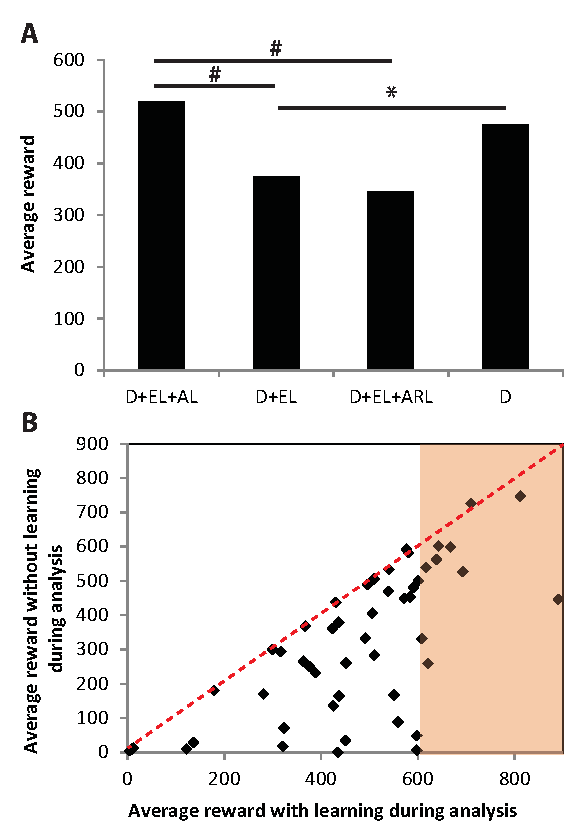
\includegraphics[width=8cm]{Fig2_Efficiency_analysis.eps}
%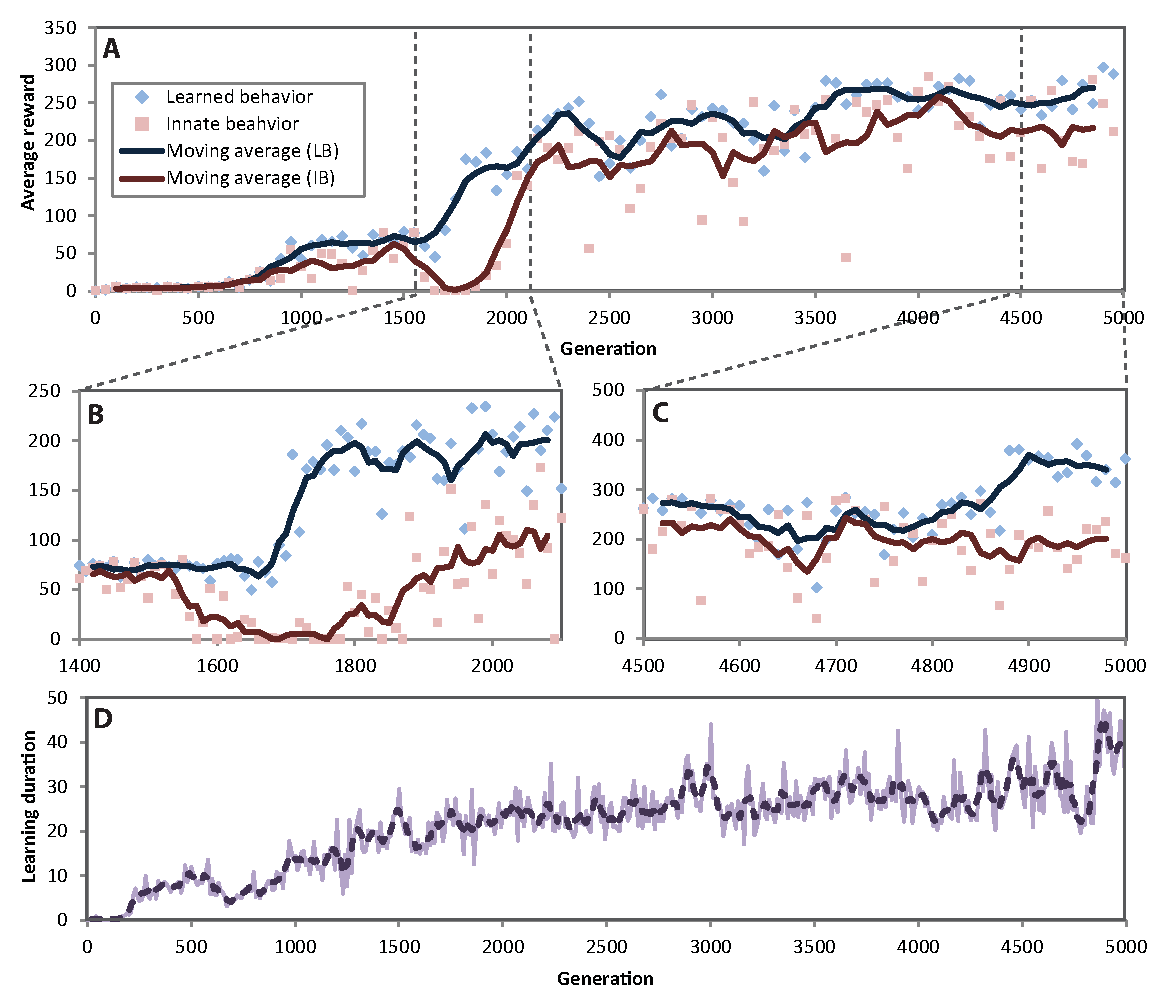
\epsfig{file=Fig3_Behavior_Evolution.eps, width=17cm}
\caption{Efficiency analysis}
\label{Efficiency_analysis}
\end{center}
\end{figure}

\begin{figure}[!b]
\begin{center}
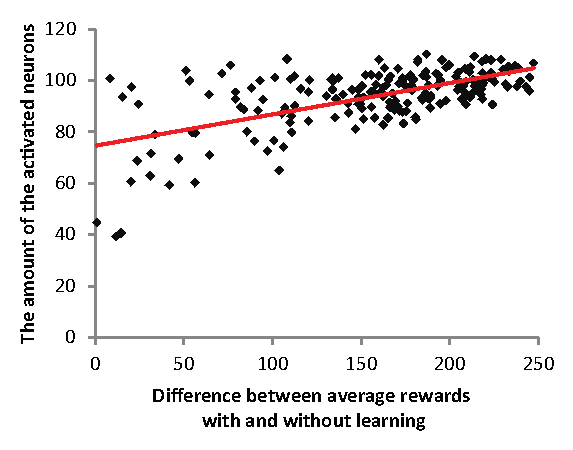
\includegraphics[width=8cm]{Fig5.eps}
%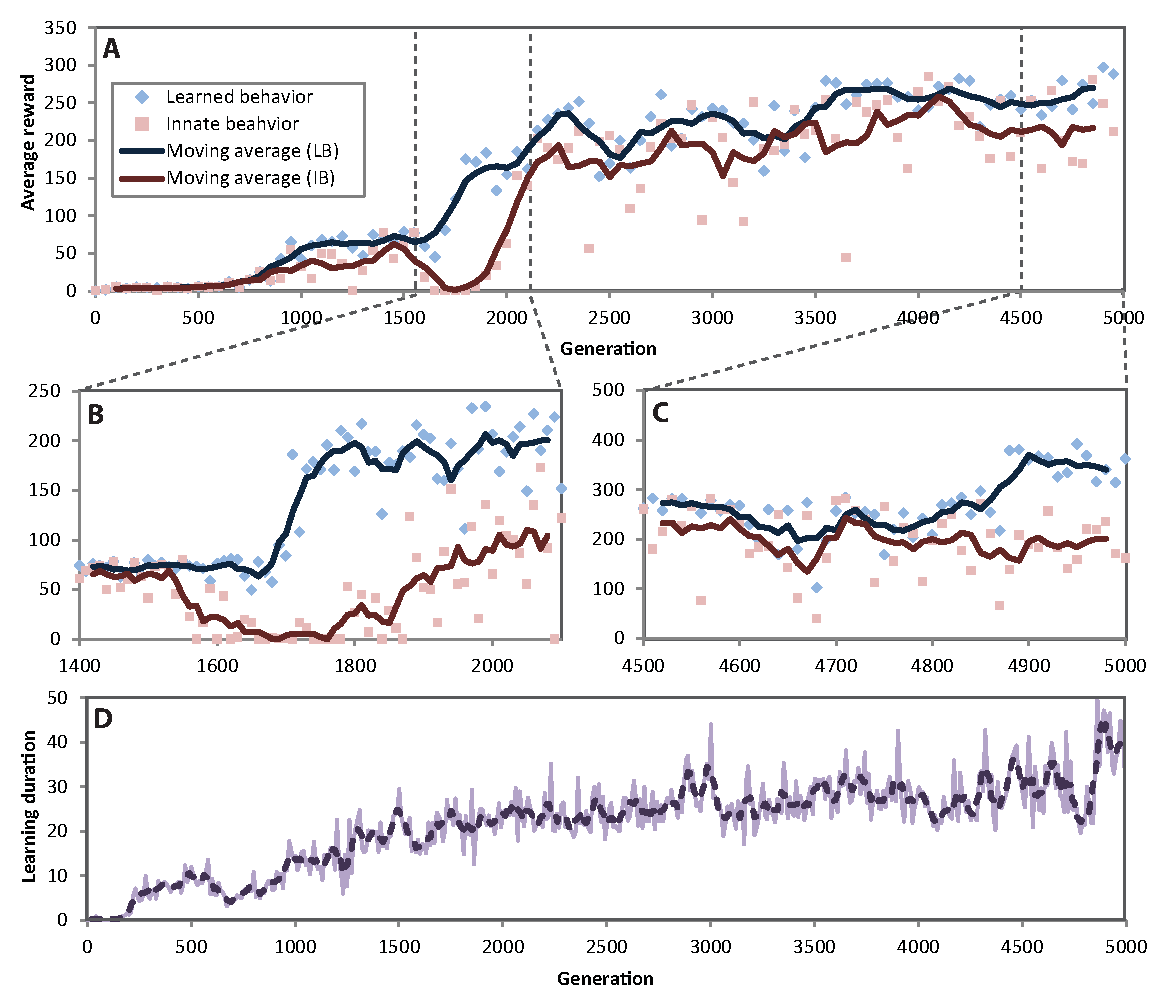
\epsfig{file=Fig3_Behavior_Evolution.eps, width=17cm}
\caption{Effectiveness analysis}
\label{Effectiveness_analysis}
\end{center}
\end{figure}


\section{Conclusions}

% \begin{figure*}[!t]
% \begin{center}
% 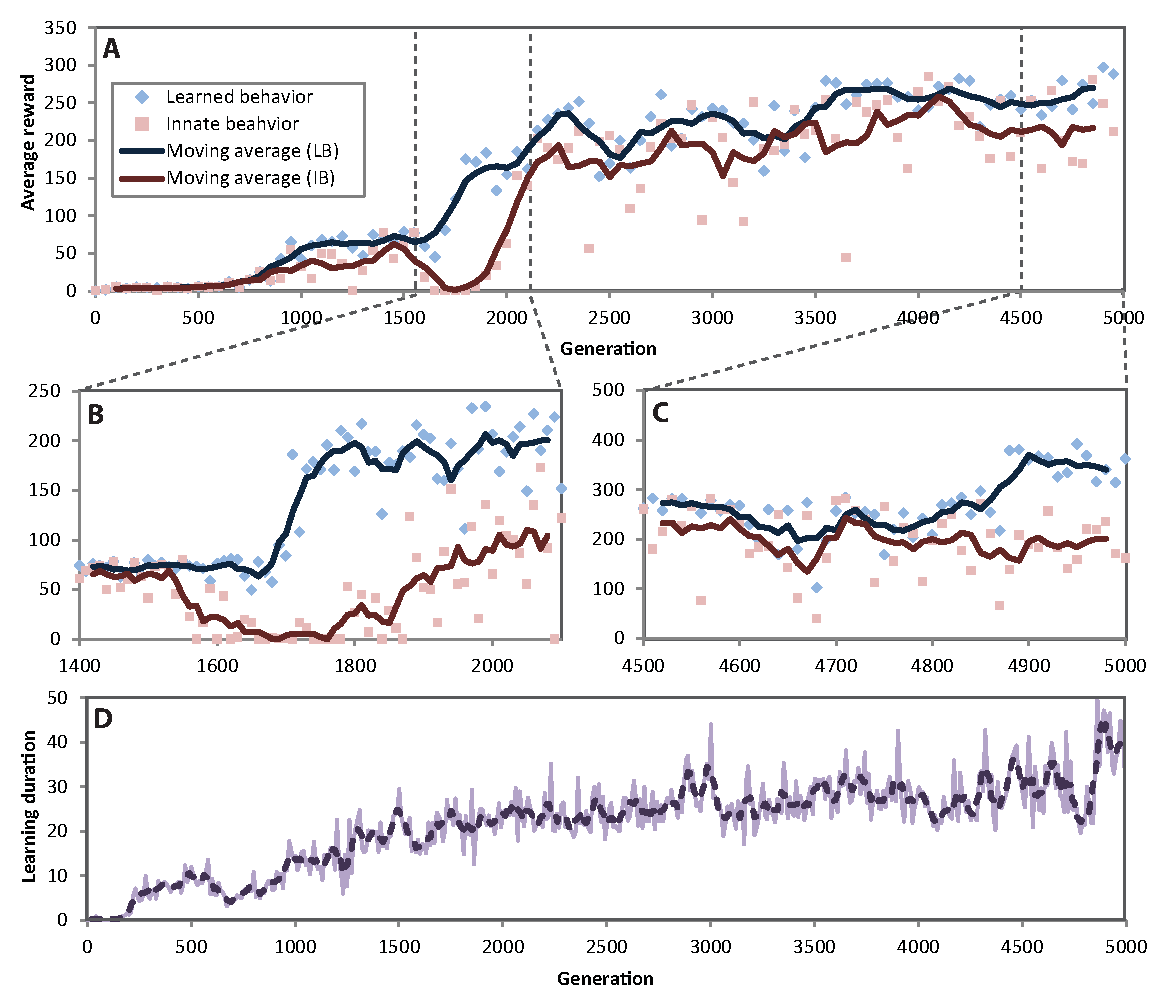
\includegraphics[width=16cm]{Fig3_Behavior_Evolution.eps}
% %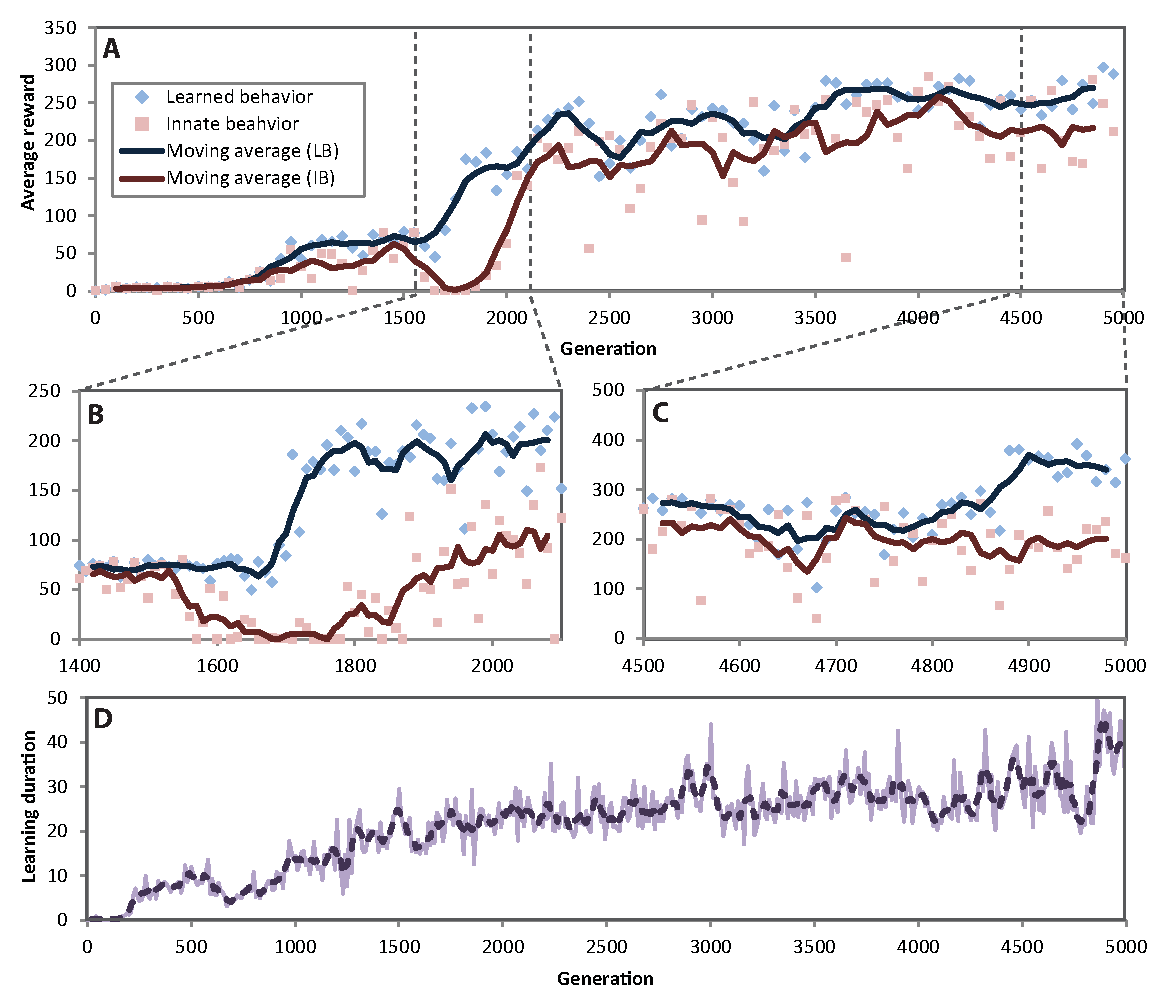
\epsfig{file=Fig3_Behavior_Evolution.eps, width=17cm}
% \caption{Behavior Evolution}
% \label{Beahvior_Evolution}
% \end{center}
% \end{figure*}

\bibliographystyle{apalike}
\bibliography{ALIFE14_paper}

\end{document}
